%!TEX root = main.tex

\section{Kapitel 4: Arrays, Dynamische Speicherverwaltung\hfill}
\label{sec:abschnitt}

% Unterabschnitt: Arrays:Vektoren

\subsection{Arrays: Vektoren\hfill}
\label{sec:unterabschnitt}

\subsubsection{Problemstellung\hfill}
\label{sec:unterunterabschnitt}
Sie müssen 10 Messwerte (z.B. Temperaturwerte) vom Typ int speichern.
\noindent
\begin{minipage}{\linewidth}
\begin{lstlisting}
int data1;
int data2;
int data3;
int data4;
int data5;
int data6;
int data7;
int data8;
int data9;
int data10;
\end{lstlisting}
\end{minipage}

Diese Darstellung ist sehr unhandlich.\\
Wie würden sie 1000 Messwerte abspeichern?

\subsubsection{Der Array (Feld, Vektor)\hfill}
\label{sec:unterunterabschnitt}
Ein Array bietet eine kompakte Zusammenfassung von mehreren Variablen des gleichen Typs.
\noindent
\begin{minipage}{\linewidth}
\begin{lstlisting}
int data[10];	// ein Array von 10 int-Werten
int data[1000];	// ein Array von 1000 int-Werten
double zahl[5];	// ein Array von 5 double-Werten
\end{lstlisting}
\end{minipage}

\subsubsection{Zugriff auf ein Arrayelement\hfill}
\label{sec:unterunterabschnitt}
\begin{hinweis}
Der Zugriff auf ein Element eines Arrays erfolgt über den Array-Index. Ist ein Array mit n Elementen definiert, so ist darauf zu achten, dass in C++ (wie in C) der Index mit 0 beginnt und mit n-1 endet.
\end{hinweis}
\noindent
\begin{minipage}{\linewidth}
\begin{lstlisting}
int alpha[5];	// der Array 'alpha' mit 5 Elementen vom Typ
	// int wird definiert
alpha[0] = 14;	// 1. Element (Index 0) wird auf 14 gesetzt
alpha[4] = 3;	// das letzte Element (Index 4)

alpha[5] = 4;	\color{\ownRed}// Bereichsueberschreitung (geht in C++!)\color{black}
\end{lstlisting}
\end{minipage}

% Unterabschnitt: Arrays und Pointer

\subsection{Arrays und Pointer\hfill}
\label{sec:unterabschnitt}

\subsubsection{Pro Memoria: Eindimensionales Array (Vektor)\hfill}
\label{sec:unterunterabschnitt}
\noindent
\begin{minipage}{\linewidth}
\begin{lstlisting}
int alpha[5];
int* ptr;
ptr = &alpha[2];
*ptr = 3452;
\end{lstlisting}
\end{minipage}

\begin{figure}[h]
	\centering
	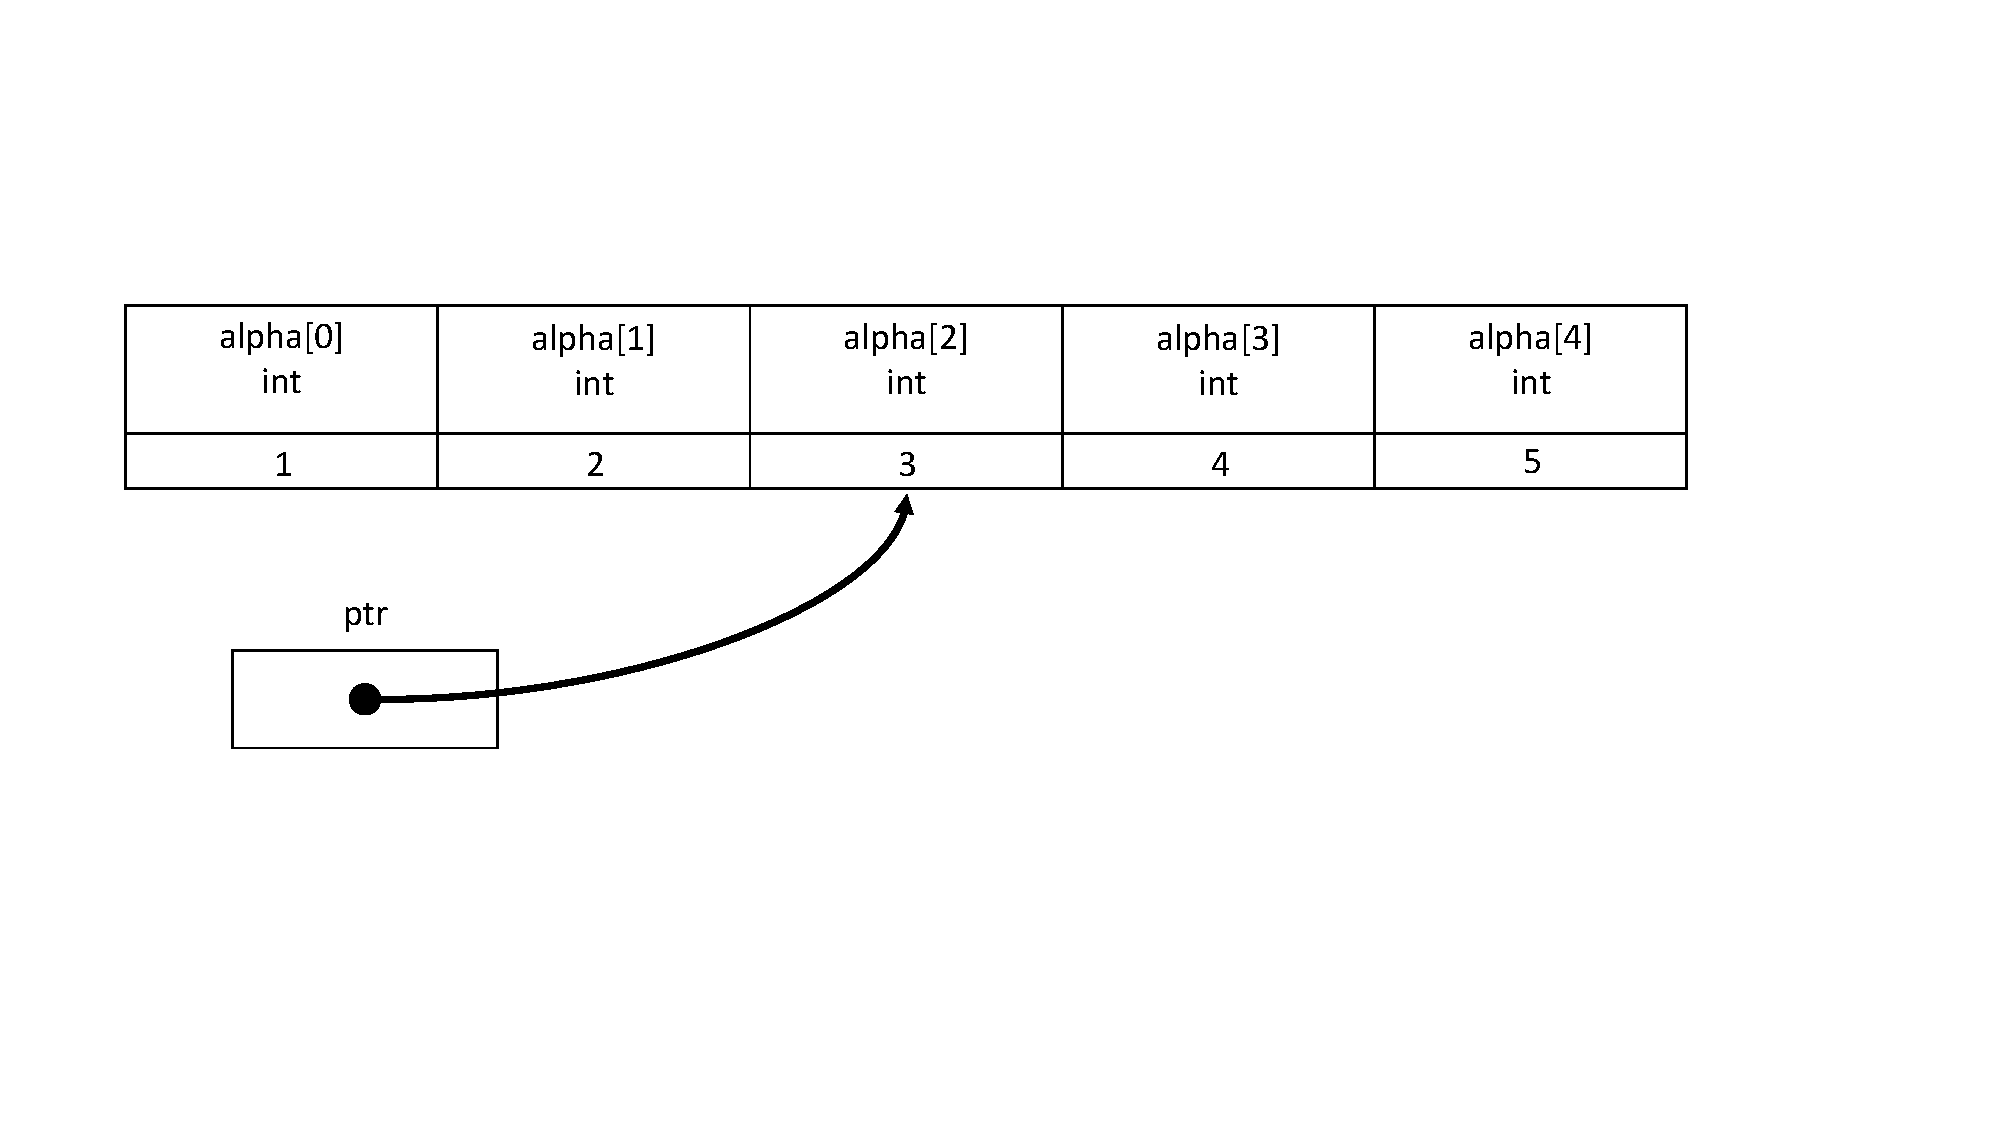
\includegraphics[width=\linewidth]{pointer9.pdf}
\end{figure}

\subsubsection{Äquivalenz von Array- und Pointernotation\hfill}
\label{sec:unterunterabschnitt}
Der Name des Array kann als konstante Adresse des ersten (Index 0) Elementes des Arrays betrachtet werden.\\
\vspace{5mm}
\begin{figure}[h]
	\centering
	%!TEX root = main.tex

\begin{tikzpicture}
	\node[draw, fit={(0,3.5) (2.5,4.5)}, inner sep=0pt, label=center:alpha{[0]}] (A) {};	% upper rectangles
	\node[draw, fit={(2.5,3.5) (5,4.5)}, inner sep=0pt, label=center:alpha{[1]}] (B) {};
	\node[draw, fit={(5,3.5) (7.5,4.5)}, inner sep=0pt, label=center:alpha{[2]}] (C) {};
	\node[draw, fit={(7.5,3.5) (10,4.5)}, inner sep=0pt, label=center:alpha{[3]}] (D) {};
	\node[draw, fit={(10,3.5) (12.5,4.5)}, inner sep=0pt, label=center:alpha{[4]}] (E) {};

	\draw[-Latex] (-.5,3) node[below] {$alpha$}  -- (A);						% pointers
	\draw[-Latex] (4.5,3) node[below] {$\&alpha[2]$} -- (C);
	
	\node[draw, fit={(7.5,1.625) (12.5,2.825)}, fill=gray!50, inner sep=0pt, label=center:alpha{[i]}{==}*(alpha + i)] () {};	% textbox
	
	\node[draw, fit={(0,0) (2.5,1)}, inner sep=0pt, label=center:*alpha] (F) {};	% lower rectangles
	\node[draw, fit={(2.5,0) (5,1)}, inner sep=0pt, label=center:*(alpha+1)] (G) {};
	\node[draw, fit={(5,0) (7.5,1)}, inner sep=0pt, label=center:*(alpha+2)] (H) {};
	\node[draw, fit={(7.5,0) (10,1)}, inner sep=0pt, label=center:*(alpha+3)] (I) {};
	\node[draw, fit={(10,0) (12.5,1)}, inner sep=0pt, label=center:*(alpha+4)] (J) {};
	
	\draw[-Latex] (-.5,1.5) node[above] {$alpha$} -- (F);
\end{tikzpicture}
\end{figure}

\subsubsection{Vergleichen von Arrays\hfill}
\label{sec:unterunterabschnitt}
\begin{itemize}
	\item\color{\ownRed}In C++ gibt es keinen Operator ==, der zwei Arrays miteinander vergleicht\color{black}
	\item Arrayvergleiche müssen explizit Element um Element durchgeführt werden
	\item oder: der Inhalt der beiden Speicherbereiche wird mit Hilfe der Funktion memcmp() byteweise verglichen
	\item Beispiel:\\Seien arr1 und arr2 zwei Arrays\\Der Vergleich arr1 == arr2 prüft, ob die Anfangsadressen der beiden Arrays identisch sind (wird kaum der Fall sein), nicht aber, ob deren Inhalte identisch sind.
\end{itemize}
	
\subsubsection{Arrayname ist ein nicht modifizierbarer L-Wert\hfill}
\label{sec:unterunterabschnitt}
\begin{itemize}
	\item Der Arrayname ist die konstante Adresse des ersten Elementes des Arrays und kann nicht verändert werden
	\item Auf den Arraynamen können nur die beiden Operatoren sizeof und \& angewandt werden
	\item Der Arrayname (z.B. arr), als auch der Adressoperator angewandt auf den Arraynamen (\&arr) ergeben einen konstanten Pointer auf das erste Element des Arrays, der Typ ist jedoch verschieden
	\item Einem Arraynamen kann kein Wert zugewiesen werden (einer Pointervariablen schon)
\end{itemize}

\subsubsection{Automatische Initialisierung von Arrays\hfill}
\label{sec:unterunterabschnitt}
\begin{itemize}
	\item Globale Arrays werden automatisch mit 0 initialisiert
	\begin{itemize}
		\item globale Arrays sollten aber nur ausnahmsweise verwendet werden
	\end{itemize}
	\item Lokale Arrays werden nicht automatisch initialisiert
	\begin{itemize}
		\item der Inhalt eines lokalen Arrays ist bei der Definition undefiniert
	\end{itemize}
\end{itemize}

\subsubsection{Explizite Initialisierung von Arrays\hfill}
\label{sec:unterunterabschnitt}
\begin{itemize}
	\item Bei der Definition eines Arrays kann ein Array explizit (''manuell'') initialisiert werden
	\item Der Definition folgt ein Zuweisungsoperator und eine Liste von Initialisierungswerten
	\item Die Liste ist mit geschweiften Klammer begrenzt
	\item Als Werte können nur Konstanten oder Ausdrücke mit Konstanten angegeben werden, \color{\ownRed}Variablen sind nicht möglich\color{black}
	\item Die Werte werden mit Kommata getrennt
	\item Nach der Initialisierung können die Elemente nur noch einzeln geändert werden
\end{itemize}

\subsubsection{Beispiel: Explizite Initialisierung von Arrays\hfill}
\label{sec:unterunterabschnitt}
\noindent
\begin{minipage}{\linewidth}
\begin{lstlisting}
in alpha[3] = {1, 2*5, 3};
\end{lstlisting}
\end{minipage}
ist ''äquivalent'' zu:
\noindent
\begin{minipage}{\linewidth}
\begin{lstlisting}
int alpha [3];

alpha[0] = 1;
alpha[1] = 2*5;
alpha[2] = 3;
\end{lstlisting}
\end{minipage}

\subsubsection{Goodies für die explizite Initialisierung\hfill}
\label{sec:unterunterabschnitt}
\begin{itemize}
	\item Werden bei der Initialisierung weniger Werte angegeben als der Array Elemente hat, so werden die restlichen Elemente mit 0 belegt.\\
	\noindent
	\begin{minipage}{\linewidth}
	\begin{lstlisting}
	int alpha[200] = {3, 105, 17};
	// alpha[3] bis alpha[199] werden gleich 0 gesetzt
	\end{lstlisting}
	\end{minipage}
	\item wird bei der Definition keine Arraygrösse angegeben, so zählt der Compiler die Anzahl Elemente automatisch (offenes Array ohne Längenangabe)
	\noindent
	\begin{minipage}{\linewidth}
	\begin{lstlisting}
	int alpha[] = {1, 2, 3, 4};
	\end{lstlisting}
	\end{minipage}
\end{itemize}

% Unterabschnitt: Mehrdimensionale Arrays

\subsection{Mehrdimensionale Arrays\hfill}
\label{sec:unterabschnitt}
\noindent
\begin{minipage}{\linewidth}
\begin{lstlisting}
int alpha[3][4];
\end{lstlisting}
\end{minipage}

\textbf{Matrix}\\
Kann betrachtet werden als Vektor alpha[0] bis alpha[2], wobei jedes Vektorelement wiederum einen Vektor mit 4 Elementen enthält\\
\vspace{5mm}
\begin{figure}[h]
	\centering
	%!TEX root = main.tex

\begin{tikzpicture}
	\node[draw, fit={(-7,0) (-5,1)}, inner sep=0pt, label=center:alpha{[2]}] (A) {};	% row
	\node[draw, fit={(-7,1) (-5,2)}, inner sep=0pt, label=center:alpha{[1]}] (B) {};
	\node[draw, fit={(-7,2) (-5,3)}, inner sep=0pt, label=center:alpha{[0]}] (C) {};	

	\node[draw, fit={(0,0) (1.5,1)}, inner sep=0pt, label=center:{[2][0]}] (AA) {};	% matrix
	\node[draw, fit={(1.5,0) (3,1)}, inner sep=0pt, label=center:{[2][1]}] (AB) {};
	\node[draw, fit={(3,0) (4.5,1)}, inner sep=0pt, label=center:{[2][2]}] (AC) {};
	\node[draw, fit={(4.5,0) (6,1)}, inner sep=0pt, label=center:{[2][3]}] (AD) {};
	\node[draw, fit={(0,1) (1.5,2)}, inner sep=0pt, label=center:{[1][0]}] (BA) {};
	\node[draw, fit={(1.5,1) (3,2)}, inner sep=0pt, label=center:{[1][1]}] (BB) {};
	\node[draw, fit={(3,1) (4.5,2)}, inner sep=0pt, label=center:{[1][2]}] (BC) {};
	\node[draw, fit={(4.5,1) (6,2)}, inner sep=0pt, label=center:{[1][3]}] (BD) {};
	\node[draw, fit={(0,2) (1.5,3)}, inner sep=0pt, label=center:{[0][0]}] (CA) {};
	\node[draw, fit={(1.5,2) (3,3)}, inner sep=0pt, label=center:{[0][1]}] (CB) {};	
	\node[draw, fit={(3,2) (4.5,3)}, inner sep=0pt, label=center:{[0][2]}] (CC) {};
	\node[draw, fit={(4.5,2) (6,3)}, inner sep=0pt, label=center:{[0][3]}] (CD) {};
	
	\draw[-Latex] (-1,2.5) node[left] {$Zeilenindex$}  -- (.4,2.5);						% pointers
	\draw[-Latex] (1,4) node[above] {$Spaltenindex$} -- (1,2.75);
\end{tikzpicture}
\end{figure}

\subsubsection{Initialisierung eines mehrdimensionalen Arrays\hfill}
\label{sec:unterunterabschnitt}
\noindent
\begin{minipage}{\linewidth}
\begin{lstlisting}
int alpha[3][4] = {
	{1, 3, 5, 7},
	{2, 4, 6, 8},
	{3, 5, 7, 9}
	};
// aequivalent dazu ist die folgende Definition:
int alpha[3][4] = {1, 3, 5, 7, 2, 4, 6, 8, 3, 5, 7, 9};
\end{lstlisting}
\end{minipage}
\\
\centering
\begin{tabularx}{0.25\textwidth}{|X|X|X|X|}
	\hline
	1 & 3 & 5 & 7\\
	\hline
	2 & 4 & 6 & 8\\
	\hline
	3 & 5 & 7 & 9\\
	\hline
\end{tabularx}
\flushleft
\begin{hinweis}
	Das erste Element kann offen sein, das zweite muss angegeben werden.
\end{hinweis}


% Unterabschnitt: Übergabe von Arrays und Zeichenketten

\subsection{Übergabe von Arrays und Zeichenketten\hfill}
\label{sec:unterabschnitt}
\begin{itemize}
	\item Bei der Übergabe eines Arrays an eine Funktion wird als Argument der Arrayname übergeben. (i.e. Pointer auf erstes Element des Arrays)
	\item Der formale Parameter für die Übergabe eines eindimensionalen Arrays kann ein offenes Array sein oder ein Pointer auf den Komponententyp des Arrays.
	\item Zeichenketten sind char-Arrays und werden deshalb gemäss der oben erwähnten Punkte gehandhabt.
\end{itemize}

\subsubsection{Beispiel: Array (Vektor) als Parameter\hfill}
\label{sec:unterunterabschnitt}
\noindent
\begin{minipage}{\linewidth}
\begin{lstlisting}
enum {groesse = 3};

void init(int* alpha, int size);	// int* alpha == Pointer auf Arrayelement
void ausgabe(int alpha[], int size);	// int alpha[] == offener Array

int main()
{
	int arr[groesse];
	init(arr, sizeof(arr)/sizeof(arr[0]));	// Argument ist Name des Arrays
	ausgabe(arr, sizeof(arr)/sizeof(arr[0]));// Argument ist Name des Arrays
	return 0;
}
\end{lstlisting}
\end{minipage}

\subsubsection{Übergabe einer Matrix mittels offenem Array\hfill}
\label{sec:unterunterabschnitt}
\noindent
\begin{minipage}{\linewidth}
\begin{lstlisting}
void printMat(const double* const mat[],	// Matrix
	int m,					// Anzahl Zeilen
	int n);					// Anzahl Spalten
\end{lstlisting}
\end{minipage}
\begin{itemize}
	\item Der Aufruf erfolgt mit \hspace{5mm}printMat(matA, rows, cols); // bevorzugt\\
		oder	\hspace{3.4cm} printMat(\&matA[0], rows, cols);\\
		oder \hspace{3.4cm} printMat(\&(\&matA[0])[0], rows, cols);
	\item matA \hspace{1cm} ist vom Typ double**\\
		matA[0] \hspace{6mm} ist vom Typ double*\\
		matA[0][0] \hspace{2mm} ist vom Typ double
\end{itemize}

\subsubsection{Zeichenketten (Strings)\hfill}
\label{sec:unterunterabschnitt}
\begin{itemize}
	\item Strings sind char-Arrays, abgeschlossen mit dem Zeichen `\textbackslash0`, bzw. 0 (alles analog C)
\end{itemize}

\subsection{Dynamische Speicherverwaltung\hfill}
\label{sec:unterabschnitt}

\subsubsection{Pro Memoria: Variablen\hfill}
\label{sec:unterunterabschnitt}
\begin{itemize}
	\item Variablen erleichtern u.a. den Zugriff auf Speicherstellen
	\begin{itemize}
		\item statt über eine Adresse kann auf die Speicherstelle mit Hilfe des Variablennamens zugegriffen werden
	\end{itemize}
	\item Die Variablen müssen zur Entwicklungszeit im Code definiert werden
	\begin{itemize}
		\item zur Laufzeit können keine neuen Variablen erzeugt werden
		\item der gesamte Speicherbedarf muss zur Entwicklungszeit statisch mittels Variablen festgelegt werden
		\item wie gross wähle ich z.B. einen Array, welcher Messwerte enthält?
		\item weiss ich zur Entwicklungszeit bereits die zahl der Messwerte?
	\end{itemize}
	\item Der Speicher einer Variablen wird automatisch freigegeben, sobald die Variable nicht mehr gültig ist
\end{itemize}

\subsubsection{Dynamische Speicherverwaltung\hfill}
\label{sec:unterunterabschnitt}
\begin{itemize}
	\item Speicher kann zur Laufzeit (dynamisch) vom System angefordert werden
	\begin{itemize}
		\item Operator: new (in C: Funktion malloc())
	\end{itemize}
	\item Dynamisch allozierter Speicher muss wieder explizit freigegeben werden
	\begin{itemize}
		\item Operator: delete (in C: Funktion free())
	\end{itemize}
	\item Dynamischer Speicher wird nicht auf dem Stack angelegt, sondern auf dem \textbf{Heap}
	\item Auf dynamischen Speicher kann \textbf{nur über Pointer} zugegriffen werden
\end{itemize}
\begin{achtung}
Zugriff auf dynamischen Speicher nie verlieren!
\end{achtung}

\subsubsection{Dynamische Speicherverwaltung: Syntax\hfill}
\label{sec:unterunterabschnitt}
\noindent
\begin{minipage}{\linewidth}
\begin{lstlisting}
int* pint = new int;	// Speicher fuer int alloziert
char* pCh1 = new char;	// Speicher fuer char alloziert
char* pCh2 = new char;	// Speicher fuer char alloziert

*pInt = 23;
std::cin >> *pCh1;
pCh2 = pCh1;
*@\color{\ownRed}// pCh2 zeigt nun auch auf die Speicherstelle, auf welche pCh1 zeigt.@*
*@\color{\ownRed}// Damit geht aber der Zugriff auf die Speicherstelle verloren, auf die pCh2 gezeigt hat@*
*@\color{\ownRed}\hspace{5mm}(Memory Leak!)@*

delete pInt;	// Speicher wieder freigeben
delete pCh1;
delete pCh2;	*@\color{\ownRed}// ergibt Fehler, bereits über pCh1 freigegeben@*
\end{lstlisting}
\end{minipage}

\subsubsection{Dynamische Speicherverwaltung: Vorsichtsmassnahmen\hfill}
\label{sec:unterunterabschnitt}
\begin{itemize}
	\item der delete-Operator kann auch auf den Nullpointer angewendet werden. Es passiert dadurch (definiert) nichts.
	\item Die Anwendung des delete-Operators auf einen  bereits freigegebenen Speicherbereich kann Probleme verursachen
	\item Oft wird deshalb eine Pointer nach der delete-Operation auf 0 gesetzt (defensiver Programmierstil)
\end{itemize}
\noindent
\begin{minipage}{\linewidth}
\begin{lstlisting}
delete pInt;	// Speicher wieder freigeben
delete pInt;	// Speicher ist bereits freigegeben
pInt = 0;
delete pInt;	// ist problemlos
\end{lstlisting}
\end{minipage}

\subsubsection{Memory Leak, Garbage Collection\hfill}
\label{sec:unterunterabschnitt}
\begin{itemize}
	\item Dynamisch allozierter Speicher, welcher nicht freigegeben wurde oder auf welchen der Zugriff verloren ging, belegt weiterhin Platz im Speicher.
	\item Der faktisch nutzbare Speicher wird somit immer kleiner. Es ist, als ob der Speicher ein Leck hätte. Dieses Fehlverhalten wird deshalb als \textbf{Memory Leak} bezeichnet.
	\item In einigen Programmiersprachen (z.B. Java) gibt es einen \textbf{Garbage Collector} (Abfalleimer), welcher nicht mehr benötigten Speicher automatisch freigibt.
	\item C++ besitzt keinen Garbage Collector. Der C++-Programmierer ist verantwortlich, dass allozierter Speicher wieder freigegeben wird.
\end{itemize}

\subsubsection{Dynamische Allozierung von Arrays\hfill}
\label{sec:unterunterabschnitt}
\begin{itemize}
	\item In C++ kann Speicher für einen Array auch erst zur Laufzeit (dynamisch) vom System angefordert (alloziert) werden
	\begin{itemize}
		\item Operator: \textbf{new[]}
	\end{itemize}
	\item Der Zugriff auf den Array erfolgt wie bei einem statischen Array
	\item Dynamisch allozierte Arrays müssen wieder explizit freigegeben werden
	\begin{itemize}
		\item Operator: \textbf{delete[]}
		\item \color{\ownRed}Achtung: delete[], nicht nur delete\color{black}
	\end{itemize}
\end{itemize}
\noindent
\begin{minipage}{\linewidth}
\begin{lstlisting}
int* pInt = new int[100];	// statt einer Konstanten kann hier auch eine Variable verwendet werden (Normalfall)
delete pInt;	*@\color{\ownRed}// Fehler: nur pInt[0] wird freigegeben\color{black}@*
delete[] pInt;	// korrekter Befehl
\end{lstlisting}
\end{minipage} 

\subsubsection{Dynamische Allozierung von Matrizen\hfill}
\label{sec:unterunterabschnitt}
\begin{itemize}
	\item Oft wird eine m x n - Matrix als ein eindimensionaler Array der Grösse (m*n) implementiert. Der Zugriff geht dann jedoch nur noch über Pointer:
	\noindent
	\begin{minipage}{\linewidth}
	\begin{lstlisting}
	*(matrix+2*n+3) = 23.44;
	\end{lstlisting}
	\end{minipage}
	\item Mit der im folgenden gezeigten Variante kann auf ein Matrixelement über die Arrayindizes zugegriffen werden:
	\begin{minipage}{\linewidth}
	\begin{lstlisting}
	matrix[2][3] = 23.44;
	\end{lstlisting}
	\end{minipage}
\end{itemize}

\subsubsection{Dynamische Matrix mit 4 Zeilen und 3 Spalten\hfill}
\label{sec:unterunterabschnitt}
\noindent
\begin{minipage}{\linewidth}
\begin{lstlisting}
double** m = 0;
\end{lstlisting}
\end{minipage}
\begin{figure}[h]
	\centering
	%!TEX root=main.tex
\begin{tikzpicture}
	\node[draw, fit={(-.5,4.5) (0,5)}, inner sep=0pt] (A) {};	% m
	\fill (-.25,4.75) circle [radius=.8mm];
	\node at (-.25,5.25) {m};
	\draw (-.25,4.75) -- (.25,4.75) -- (.25,4.25) -- (.5,4.25) -- (0,4.25);
\end{tikzpicture}
\end{figure}
\vspace{5mm};
\noindent
\begin{minipage}{\linewidth}
\begin{lstlisting}
double** m = 0;
m = new double*[4];		// Array mit 4 Elementen vom Typ double* (Pointer auf double)
\end{lstlisting}
\end{minipage}
\begin{figure}[h]
	\centering
	%!TEX root=main.tex
\begin{tikzpicture}
	\node[draw, fit={(-.5,2.5) (0,3)}, inner sep=0pt] (A) {};	% m
	\fill (-.25,2.75) circle [radius=.8mm];
	\node at (-.25,3.25) {m};

	\node[draw, fit={(0,0) (.5,.5)}, inner sep=0pt] {};	% m0-3
	\fill (.25,.25) circle [radius=.8mm];
	\node at (-.5,.25) {m{[3]}};
	\node[draw, fit={(0,.5) (.5,1)}, inner sep=0pt] {};
	\fill (.25,.75) circle [radius=.8mm];
	\node at (-.5,.75) {m{[2]}};
	\node[draw, fit={(0,1) (.5,1.5)}, inner sep=0pt] {};
	\fill (.25,1.25) circle [radius=.8mm];
	\node at (-.5,1.25) {m{[1]}};
	\node[draw, fit={(0,1.5) (.5,2)}, inner sep=0pt] (B) {};
	\fill (.25,1.75) circle [radius=.8mm];
	\node at (-.5,1.75) {m{[0]}};
	
	\draw[-Latex] (-.25,2.75) -- (B);  % Pointer
\end{tikzpicture}
\end{figure}
\vspace{5mm};
\noindent
\begin{minipage}{\linewidth}
\begin{lstlisting}
double** m = 0;
m = new double*[4];		// Array mit 4 Elementen vom Typ double* (Pointer auf double)
for (int i=0; i<4; ++i)	
	m[i] = new double[3];	// Jedes m[i] ist ein Pointer auf ein Array mit 3 Elementen vom Typ double
				// m[i] selbst ist vom Typ double*	
\end{lstlisting}
\end{minipage}
\begin{figure}[hh]
	\centering
	%!TEX root=main.tex
\begin{tikzpicture}
	\node[draw, fit={(-.5,2.5) (0,3)}, inner sep=0pt] (C) {};	% m
	\fill (-.25,2.75) circle [radius=.8mm];
	\node at (-.25,3.25) {m};

	\node[draw, fit={(0,0) (.5,.5)}, inner sep=0pt] (D) {};	% m0-3
	\fill (.25,.25) circle [radius=.8mm];
	\node at (-.5,.25) {m{[3]}};
	\node[draw, fit={(0,.5) (.5,1)}, inner sep=0pt] (E) {};
	\fill (.25,.75) circle [radius=.8mm];
	\node at (-.5,.75) {m{[2]}};
	\node[draw, fit={(0,1) (.5,1.5)}, inner sep=0pt] (F) {};
	\fill (.25,1.25) circle [radius=.8mm];
	\node at (-.5,1.25) {m{[1]}};
	\node[draw, fit={(0,1.5) (.5,2)}, inner sep=0pt] (G) {};
	\fill (.25,1.75) circle [radius=.8mm];
	\node at (-.5,1.75) {m{[0]}};
	
	\node[draw, fit={(1.5,0) (3,.5)}, inner sep=0pt, label=center:m{[3][0]}] (DA) {};	% Matrix
	\node[draw, fit={(3,0) (4.5,.5)}, inner sep=0pt, label=center:m{[3][1]}] {};
	\node[draw, fit={(4.5,0) (6,.5)}, inner sep=0pt, label=center:m{[3][2]}] {};
	\node[draw, fit={(1.5,.5) (3,1)}, inner sep=0pt, label=center:m{[2][0]}] (EA) {};
	\node[draw, fit={(3,.5) (4.5,1)}, inner sep=0pt, label=center:m{[2][1]}] {};
	\node[draw, fit={(4.5,.5) (6,1)}, inner sep=0pt, label=center:m{[2][2]}] {};
	\node[draw, fit={(1.5,1) (3,1.5)}, inner sep=0pt, label=center:m{[1][0]}] (FA) {};	
	\node[draw, fit={(3,1) (4.5,1.5)}, inner sep=0pt, label=center:m{[1][1]}] {};
	\node[draw, fit={(4.5,1) (6,1.5)}, inner sep=0pt, label=center:m{[1][2]}] {};	
	\node[draw, fit={(1.5,1.5) (3,2)}, inner sep=0pt, label=center:m{[0][0]}] (GA) {};
	\node[draw, fit={(3,1.5) (4.5,2)}, inner sep=0pt, label=center:m{[0][1]}] {};	
	\node[draw, fit={(4.5,1.5) (6,2)}, inner sep=0pt, label=center:m{[0][2]}] {};
	
	\draw[-Latex] (-.25,2.75) -- (G);  % Pointer
	\draw[-Latex] (.25,.25) -- (DA);
	\draw[-Latex] (.25,.75) -- (EA);
	\draw[-Latex] (.25,1.25) -- (FA);
	\draw[-Latex] (.25, 1.75) -- (GA);
\end{tikzpicture}
\end{figure}
\\
Für die Konstanten 3 und 4 könnten auch Variablen verwendet werden (im Gegensatz zu einer statisch definierten Matrix).

\subsubsection{Zugriff auf dynamisch erzeugte Matrix\hfill}
\label{sec:unterunterabschnitt}
\noindent
\begin{minipage}{\linewidth}
\begin{lstlisting}
double** m = 0;
m = new double*[4];
for (int i=0; i<4; ++i)	
	m[i] = new double[3];	
m[2][1] = 34.675;	// Der Zugriff erfolgt einfach ueber die Arrayindizes	
\end{lstlisting}
\end{minipage}
\begin{figure}[hh]
	\centering
	%!TEX root=main.tex
\begin{tikzpicture}
	\node[draw, fit={(-.5,2.5) (0,3)}, inner sep=0pt] (C) {};	% m
	\fill (-.25,2.75) circle [radius=.8mm];
	\node at (-.25,3.25) {m};

	\node[draw, fit={(0,0) (.5,.5)}, inner sep=0pt] (D) {};	% m0-3
	\fill (.25,.25) circle [radius=.8mm];
	\node at (-.5,.25) {m{[3]}};
	\node[draw, fit={(0,.5) (.5,1)}, inner sep=0pt] (E) {};
	\fill (.25,.75) circle [radius=.8mm];
	\node at (-.5,.75) {m{[2]}};
	\node[draw, fit={(0,1) (.5,1.5)}, inner sep=0pt] (F) {};
	\fill (.25,1.25) circle [radius=.8mm];
	\node at (-.5,1.25) {m{[1]}};
	\node[draw, fit={(0,1.5) (.5,2)}, inner sep=0pt] (G) {};
	\fill (.25,1.75) circle [radius=.8mm];
	\node at (-.5,1.75) {m{[0]}};
	
	\node[draw, fit={(1.5,0) (3,.5)}, inner sep=0pt, label=center:m{[3][0]}] (DA) {};	% Matrix
	\node[draw, fit={(3,0) (4.5,.5)}, inner sep=0pt, label=center:m{[3][1]}] {};
	\node[draw, fit={(4.5,0) (6,.5)}, inner sep=0pt, label=center:m{[3][2]}] {};
	\node[draw, fit={(1.5,.5) (3,1)}, inner sep=0pt, label=center:m{[2][0]}] (EA) {};
	\node[draw, fit={(3,.5) (4.5,1)}, inner sep=0pt, label=center:m{[2][1]}, fill=blue!40!white] {};
	\node[draw, fit={(4.5,.5) (6,1)}, inner sep=0pt, label=center:m{[2][2]}] {};
	\node[draw, fit={(1.5,1) (3,1.5)}, inner sep=0pt, label=center:m{[1][0]}] (FA) {};	
	\node[draw, fit={(3,1) (4.5,1.5)}, inner sep=0pt, label=center:m{[1][1]}] {};
	\node[draw, fit={(4.5,1) (6,1.5)}, inner sep=0pt, label=center:m{[1][2]}] {};	
	\node[draw, fit={(1.5,1.5) (3,2)}, inner sep=0pt, label=center:m{[0][0]}] (GA) {};
	\node[draw, fit={(3,1.5) (4.5,2)}, inner sep=0pt, label=center:m{[0][1]}] {};	
	\node[draw, fit={(4.5,1.5) (6,2)}, inner sep=0pt, label=center:m{[0][2]}] {};
	
	\draw[-Latex] (-.25,2.75) -- (G);  % Pointer
	\draw[-Latex] (.25,.25) -- (DA);
	\draw[-Latex] (.25,.75) -- (EA);
	\draw[-Latex] (.25,1.25) -- (FA);
	\draw[-Latex] (.25, 1.75) -- (GA);
\end{tikzpicture}
\end{figure}
\vspace{1cm}
\\

\subsubsection{Dynamische Matrix freigeben\hfill}
\label{sec:unterunterabschnitt}
\noindent
\begin{minipage}{\linewidth}
\begin{lstlisting}
for(int i=0; i<4; ++i)
	delete[] m[i]	// Zuerst jede Zeile freigeben		
\end{lstlisting}
\end{minipage}
\begin{figure}[hh]
	\centering
	%!TEX root=main.tex	
\begin{tikzpicture}
	\node[draw, fit={(-.5,2.5) (0,3)}, inner sep=0pt] (C) {};	% m
	\fill (-.25,2.75) circle [radius=.8mm];
	\node at (-.25,3.25) {m};

	\node[draw, fit={(0,0) (.5,.5)}, inner sep=0pt] (D) {};	% m0-3
	\fill (.25,.25) circle [radius=.8mm];
	\node at (-.5,.25) {m{[3]}};
	\node[draw, fit={(0,.5) (.5,1)}, inner sep=0pt] (E) {};
	\fill (.25,.75) circle [radius=.8mm];
	\node at (-.5,.75) {m{[2]}};
	\node[draw, fit={(0,1) (.5,1.5)}, inner sep=0pt] (F) {};
	\fill (.25,1.25) circle [radius=.8mm];
	\node at (-.5,1.25) {m{[1]}};
	\node[draw, fit={(0,1.5) (.5,2)}, inner sep=0pt] (G) {};
	\fill (.25,1.75) circle [radius=.8mm];
	\node at (-.5,1.75) {m{[0]}};
	
	\node[draw, fit={(1.5,0) (3,.5)}, inner sep=0pt, label={[gray!40!white]center:m{[3][0]}}, color=gray!40!white] (DA) {};	% Matrix
	\node[draw, fit={(3,0) (4.5,.5)}, inner sep=0pt, label={[gray!40!white]center:m{[3][1]}}, color=gray!40!white] {};
	\node[draw, fit={(4.5,0) (6,.5)}, inner sep=0pt, label={[gray!40!white]center:m{[3][2]}}, color=gray!40!white] {};
	\node[draw, fit={(1.5,.5) (3,1)}, inner sep=0pt, label={[gray!40!white]center:m{[2][0]}}, color=gray!40!white] (EA) {};
	\node[draw, fit={(3,.5) (4.5,1)}, inner sep=0pt, label={[gray!40!white]center:m{[2][1]}}, color=gray!40!white] {};
	\node[draw, fit={(4.5,.5) (6,1)}, inner sep=0pt, label={[gray!40!white]center:m{[2][2]}}, color=gray!40!white] {};
	\node[draw, fit={(1.5,1) (3,1.5)}, inner sep=0pt, label={[gray!40!white]center:m{[1][0]}}, color=gray!40!white] (FA) {};	
	\node[draw, fit={(3,1) (4.5,1.5)}, inner sep=0pt, label={[gray!40!white]center:m{[1][1]}}, color=gray!40!white] {};
	\node[draw, fit={(4.5,1) (6,1.5)}, inner sep=0pt, label={[gray!40!white]center:m{[1][2]}}, color=gray!40!white] {};	
	\node[draw, fit={(1.5,1.5) (3,2)}, inner sep=0pt, label={[gray!40!white]center:m{[0][0]}}, color=gray!40!white] (GA) {};
	\node[draw, fit={(3,1.5) (4.5,2)}, inner sep=0pt, label={[gray!40!white]center:m{[0][1]}}, color=gray!40!white] {};	
	\node[draw, fit={(4.5,1.5) (6,2)}, inner sep=0pt, label={[gray!40!white]center:m{[0][2]}}, color=gray!40!white] {};
	
	\draw[-Latex] (-.25,2.75) -- (G);  % Pointer
	\draw[-Latex] (.25,.25) -- (DA);
	\draw[-Latex] (.25,.75) -- (EA);
	\draw[-Latex] (.25,1.25) -- (FA);
	\draw[-Latex] (.25, 1.75) -- (GA);
\end{tikzpicture}
	\\
	%!TEX root=main.tex
\begin{tikzpicture}
	\node[draw, fit={(-.5,2.5) (0,3)}, inner sep=0pt] (C) {};	% m
	\fill (-.25,2.75) circle [radius=.8mm];
	\node at (-.25,3.25) {m};

	\node[draw, fit={(0,0) (.5,.5)}, inner sep=0pt] (D) {};	% m0-3
	\fill (.25,.25) circle [radius=.8mm];
	\node at (-.5,.25) {m{[3]}};
	\node[draw, fit={(0,.5) (.5,1)}, inner sep=0pt] (E) {};
	\fill (.25,.75) circle [radius=.8mm];
	\node at (-.5,.75) {m{[2]}};
	\node[draw, fit={(0,1) (.5,1.5)}, inner sep=0pt] (F) {};
	\fill (.25,1.25) circle [radius=.8mm];
	\node at (-.5,1.25) {m{[1]}};
	\node[draw, fit={(0,1.5) (.5,2)}, inner sep=0pt] (G) {};
	\fill (.25,1.75) circle [radius=.8mm];
	\node at (-.5,1.75) {m{[0]}};
	
	\draw[-Latex] (-.25,2.75) -- (G);  % Pointer
	\draw[-Latex] (.25,.25) -- (1.5,.25);
	\draw[-Latex] (.25,.75) -- (1.5,.75);
	\draw[-Latex] (.25,1.25) -- (1.5,1.25);
	\draw[-Latex] (.25, 1.75) -- (1.5,1.75);
\end{tikzpicture}
\end{figure}
\vspace{1cm}
\noindent
\begin{minipage}{\linewidth}
\begin{lstlisting}
for(int i=0; i<4; ++i)
	delete[] m[i]

delete[] m;	// Nun noch den Array mit den double* freigeben
\end{lstlisting}
\end{minipage}
\begin{figure}[hh]
	\centering
	%!TEX root=main.tex
\begin{tikzpicture}
	\node[draw, fit={(-.5,2.5) (0,3)}, inner sep=0pt] (C) {};	% m
	\fill (-.25,2.75) circle [radius=.8mm];
	\node at (-.25,3.25) {m};

	\color{gray!40!white};
	
	\node[draw, fit={(0,0) (.5,.5)}, inner sep=0pt] (D) {};	% m0-3
	\fill (.25,.25) circle [radius=.8mm];
	\node at (-.5,.25) {m{[3]}};
	\node[draw, fit={(0,.5) (.5,1)}, inner sep=0pt] (E) {};
	\fill (.25,.75) circle [radius=.8mm];
	\node at (-.5,.75) {m{[2]}};
	\node[draw, fit={(0,1) (.5,1.5)}, inner sep=0pt] (F) {};
	\fill (.25,1.25) circle [radius=.8mm];
	\node at (-.5,1.25) {m{[1]}};
	\node[draw, fit={(0,1.5) (.5,2)}, inner sep=0pt] (G) {};
	\fill (.25,1.75) circle [radius=.8mm];
	\node at (-.5,1.75) {m{[0]}};
	
	\draw[-Latex] (.25,.25) -- (1.5,.25);	% Pointer
	\draw[-Latex] (.25,.75) -- (1.5,.75);
	\draw[-Latex] (.25,1.25) -- (1.5,1.25);
	\draw[-Latex] (.25, 1.75) -- (1.5,1.75);
	\color{black};
	\draw[-Latex] (-.25,2.75) -- (G);
\end{tikzpicture}
	\\
	%!TEX root=main.tex
\begin{tikzpicture}
	\node[draw, fit={(-.5,2.5) (0,3)}, inner sep=0pt] (C) {};	% m
	\fill (-.25,2.75) circle [radius=.8mm];
	\node at (-.25,3.25) {m};
	\draw[-Latex] (-.25,2.75) -- (0,2);
\end{tikzpicture}
\end{figure}
\\
\vspace{1cm}
\begin{achtung}
m zeigt immer noch auf die alte Adresse, an welcher sich aber keine gültigen Daten mehr befinden. (Allenfalls m wieder auf 0 setzen)
\end{achtung}

\subsubsection{Effizienz der Matriximplementationen\hfill}
\label{sec:unterunterabschnitt}
\begin{itemize}
	\item Nur mit dieser gezeigten Variante kann auf ein Matrixelement über die Arrayindizes zugegriffen werden:
	\begin{minipage}{\linewidth}
	\begin{lstlisting}
	matrix[2][3] = 23.44;
	\end{lstlisting}
	\end{minipage}
	\item Der Nachteil dieser Variante ist, dass es pro Zeile einen zusätzlichen Pointer braucht. Die einzelnen Zeilen liegen u.U. nicht auf aufeinanderfolgenden Speicherstellen.
	\item Wenn eine m x n - Matrix als ein eindimensionaler Array der Grösse (m*n) implementiert wird, erspart man sich die Zeilenpointer, der Zugriff ist jedoch langsamer und mühsamer. Die einzelnen Elemente der Matrix liegen auf aufeinanderfolgenden Speicherstellen.
\end{itemize}

% ENDE